\documentclass[xcolor=dvipsnames]{beamer} 
\usecolortheme[named=Orange]{structure} 
\usetheme{Warsaw}

\usepackage{multicol}
\usepackage{caption} % podpisy pod obrazkami
\usepackage[export]{adjustbox} % ramki dla obrazków
\usepackage{pgfplots} % wykresy
\usepackage{amsmath} % wzory funkcji

\usepackage{polski}
\usepackage[utf8x]{inputenc}

% pisanie Rys. zamiast Rysunek pod obrazkami
\renewcommand{\figurename}{Rys.}

\setbeamerfont{caption}{series=\normalfont,size=\fontsize{7}{7}}

% numerowanie slajdów
\expandafter\def\expandafter\insertshorttitle\expandafter{%
  \insertshorttitle\hfill%
\insertframenumber\,/\,\inserttotalframenumber}

% slajdy z planem każdej sekcji
\AtBeginSection[]
{
  \begin{frame}
    \frametitle{Plan prezentacji}
    \tableofcontents[currentsection]
  \end{frame}
}

% referencje
\usepackage[absolute,overlay]{textpos} 
\newenvironment{reference}[2]{% 
  \begin{textblock*}{\textwidth}(#1,#2) 
\footnotesize\it\bgroup\color{red!50!black}}{\egroup\end{textblock*}} 

\title[Metody głębokiego uczenia]{DCNN - metody głębokiego uczenia w~rozpoznawaniu obrazów}
\subtitle[]{}
\author[J. Witkowski]{Jacek Witkowski}
\institute[SMD2]{
  Prezentacja w~ramach przedmiotu: Seminarium Dyplomowe 2
}
\date[Listopad 2016]{18 listopada 2016}

\begin{document}

% strona tytułowa
\begin{frame}[plain]
  \titlepage
\end{frame}

% plan prezentacji
\begin{frame}{Plan prezentacji}
  \tableofcontents
\end{frame}

\section{Wprowadzenie}
\subsection{Czym jest uczenie maszynowe?}
\begin{frame}{Czym jest uczenie maszynowe?}
  \begin{block}{Definicje}
    \textbf{Uczenie maszynowe} -- dziedzina wchodząca w skład nauk zajmujących się problematyką Sztucznej Inteligencji.\\
    \vspace{2mm}
    \textbf{Sztuczna Inteligencja} -- dział informatyki zajmujący się inteligencją – tworzeniem modeli zachowań inteligentnych oraz programów komputerowych symulujących te zachowania.\\
    \vspace{5mm}
    \hspace*\fill{\scriptsize--- Cichosz P., Systemy uczące się, WNT Warszawa, 2000}
  \end{block}
\end{frame}

\subsection{Rozwój Sztucznej Inteligencji}
\begin{frame}{Sztuczna Inteligencja w fantastyce naukowej}
  \begin{figure}
	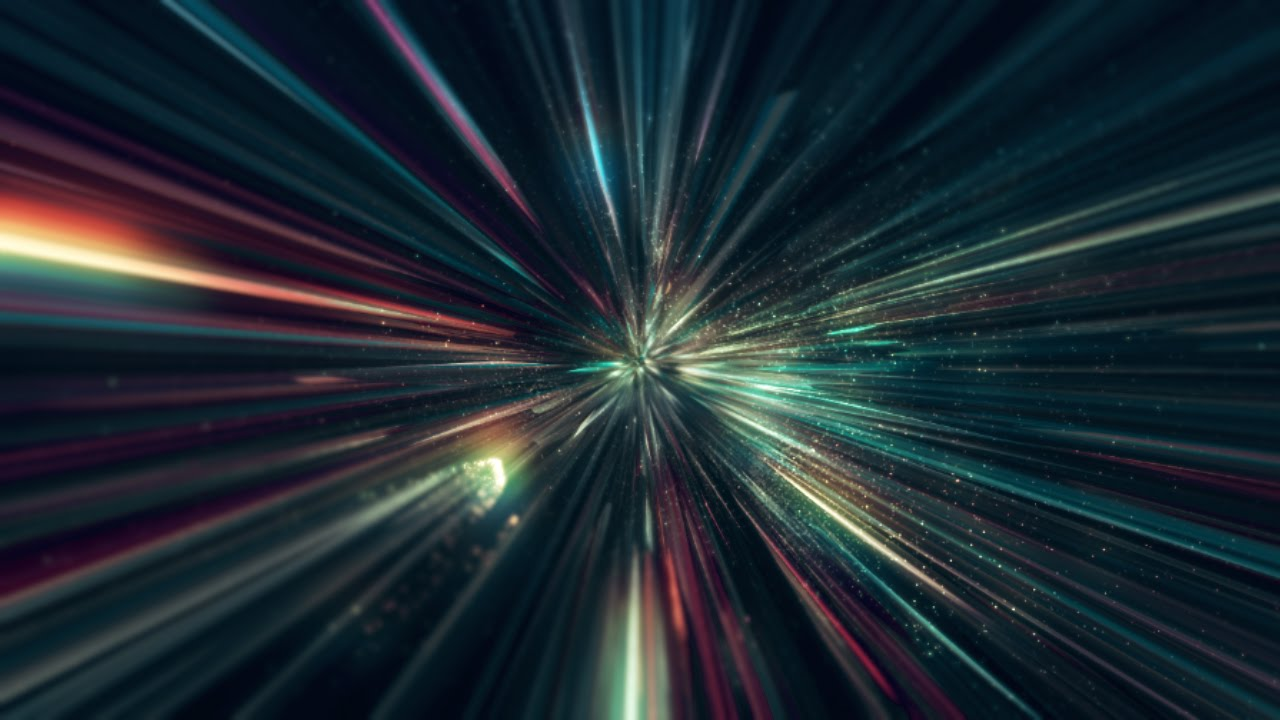
\includegraphics[width=\linewidth,height=0.8\textheight,keepaspectratio]{img/warp.jpg}
	\caption{http://3tags.org/article/will-warp-drive-finally-become-a-reality}
  \end{figure}
\end{frame}
\begin{frame}{Wzrost mocy obliczeniowej na przestrzeni lat}
 \begin{figure}
 	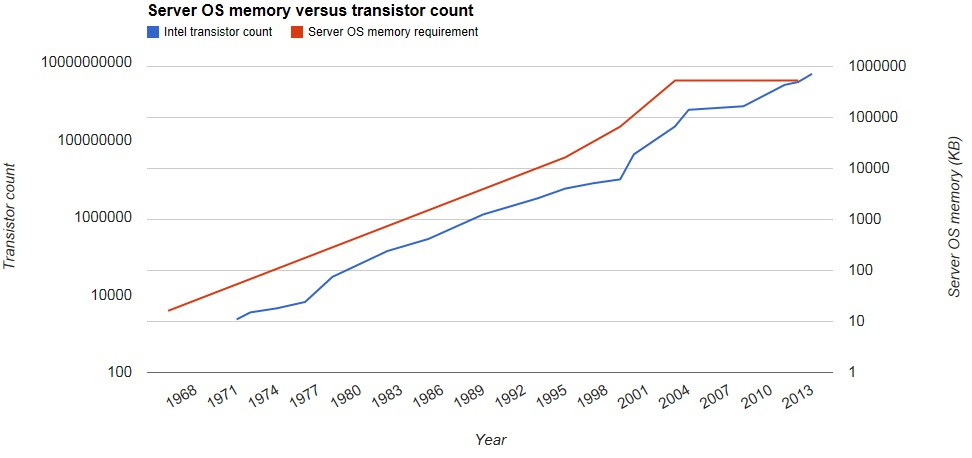
\includegraphics[width=\linewidth,height=0.8\textheight,keepaspectratio]{img/computational-power-growth.jpg}
 	\caption{http://www.forbes.com/sites/ciocentral/2014/05/19/why-software-doesnt-follow-moores-law}
  \end{figure}
\end{frame}
\begin{frame}{Problemy związane z szybkim rozwojem technologii}
	\begin{minipage}[t]{0.45\linewidth}
		Czarna wizja przyszłości:
		\begin{itemize}
			\item bezrobocie,
			\item dyktatura,
			\item zagłada ludzkości,
			\item ???
		\end{itemize}
		\vspace{5mm}	
		Problemy natury moralnej:
		\begin{itemize}
			\item samoprowadzące się samochody,
			\item roboty ratujące życie.
		\end{itemize}
	\end{minipage}%
	\hfill
	\begin{minipage}[t]{0.45\linewidth}
		\vfill
		\begin{figure}
			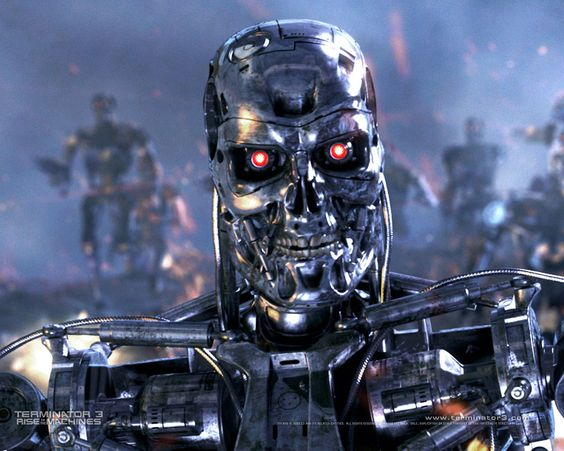
\includegraphics[width=\textwidth]{img/terminator.jpg} 
		\end{figure}
	\end{minipage}%
\end{frame}
\begin{frame}{Sieć splotowa i selfie - Andrej Karpathy blog}
  \begin{figure}
  	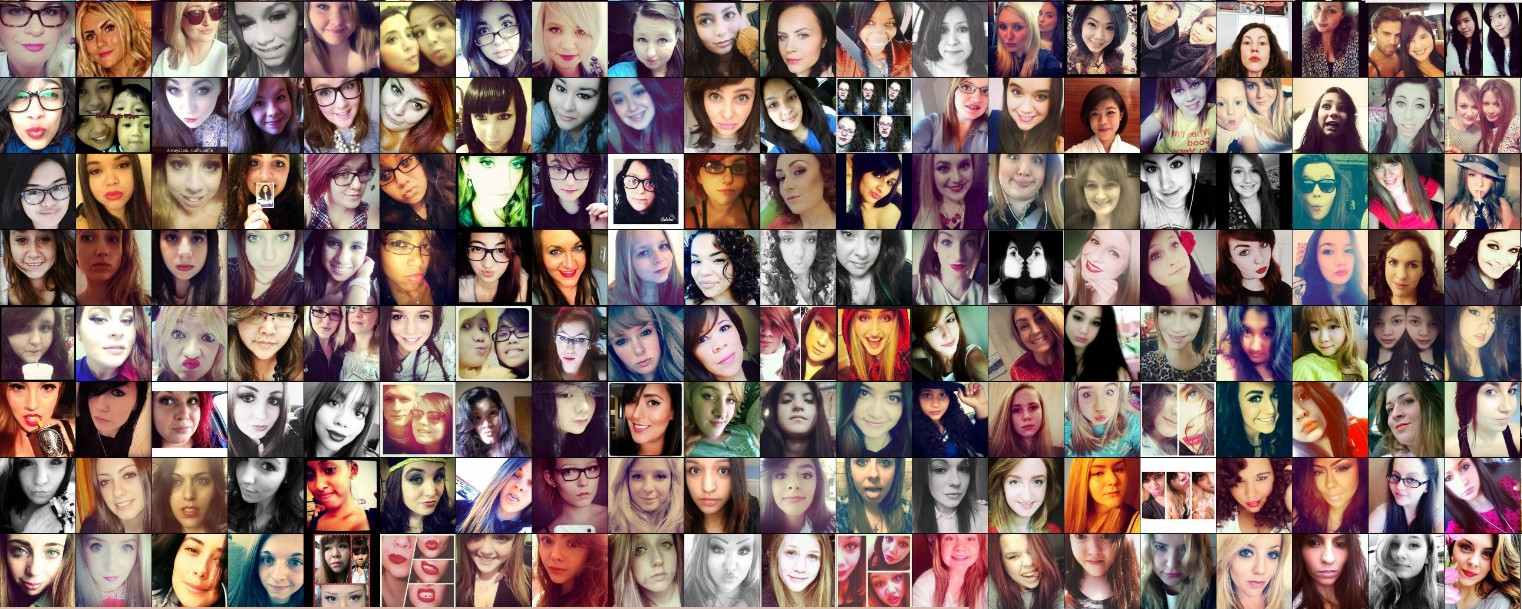
\includegraphics[width=\textwidth]{img/selfie.jpeg} 
  \end{figure}
\end{frame}
\begin{frame}{Sieć splotowa i selfie - Andrej Karpathy blog c.d.}
	\begin{enumerate}
		\item Wyszukano zdjęcia ze znacznikiem \#selfie.
		\item Przy użyciu innej sieci splotowej wybrano zdjęcia zawierające przynajmniej jedną twarz.
		\item Utworzono ranking zdjęć na podstawie liczby polubień.
		\item Poetykietowano dane na podstawie rankingu.
		\item Nauczono sieć rozpoznawać "dobre" selfie.
	\end{enumerate}
\end{frame}
\begin{frame}{Projekt Super-Resolution}
	\begin{figure}
		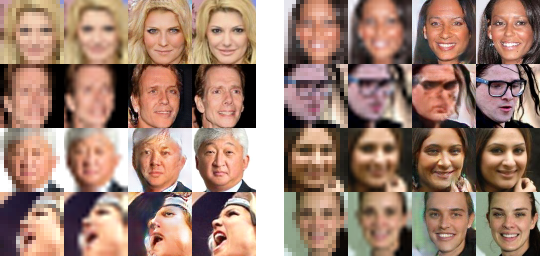
\includegraphics[width=\textwidth]{img/super-resolution.png}
	\end{figure}
\end{frame}
\begin{frame}{AlphaGo}
	\begin{figure}
		
\includegraphics[width=0.3\textwidth]{img/alpha_go.png}
	\end{figure}
	\begin{itemize}
		\item 2015 październik - pierwszy raz program komputerowy pokonuje profesjonalnego gracza Go na pełnowymiarowej planszy 19x19 (Fan Hui: 2. dan, mistrz Europy),
		\item 2016 marzec - pokonanie Lee Sedola, 18-krotnego mistrza świata, zawodnika z 9. danem (najwyższy możliwy stopień w~Go),
		\item żadna popularna gra planszowa (szachy, warcaby, Go) nie stanowi już więcej problemu dla Sztucznej Inteligencji.
	\end{itemize}
\end{frame}

\section{Uczenie maszynowe}
\subsection{Typy uczenia maszynowego}
\begin{frame}{Typy uczenia maszynowego}
	Podział ze względu na rodzaj informacji dostarczonej w zbiorze przykładów:
	\begin{itemize}
		\item uczenie nadzorowane,
		\item uczenie nienadzorowane.
	\end{itemize}
\end{frame}
\begin{frame}{Uczenie nadzorowane}
  \begin{block}{Definicja}
  	\textbf{Uczenie nadzorowane} --  uczenie maszynowe, które zakłada obecność ludzkiego nadzoru nad tworzeniem funkcji odwzorowującej wejście systemu na jego wyjście.\\
  	\vspace{5mm}
  	\hspace*\fill{\scriptsize https://pl.wikipedia.org/wiki/Uczenie\_nadzorowane}
  \end{block}
\end{frame}
\begin{frame}{Uczenie nienadzorowane}
	\begin{block}{Definicja}
		 \textbf{Uczenie nienadzorowane} --  uczenie maszynowe, które zakłada brak obecności dokładnego lub nawet przybliżonego wyjścia w danych uczących.\\
		\vspace{5mm}
		\hspace*\fill{\scriptsize https://pl.wikipedia.org/wiki/Uczenie\_nienadzorowane}
	\end{block}	
\end{frame}
\subsection{Uczenie wstępne}
\begin{frame}{Połączenie obu typów uczenia - przykład}
	\begin{minipage}[t]{0.45\linewidth}
		Rozpoznawanie jabłek:
		\begin{enumerate}
			\item Obserwacja dużego zbioru jabłek, które nie~są~opisane (uczenie wstępne).
			\item Obserwacja zbioru jabłek, które są opisane.
		\end{enumerate}
		\vspace{5mm}	
	\end{minipage}%
	\hfill
	\begin{minipage}[t]{0.45\linewidth}
		\vfill
		\begin{figure}
			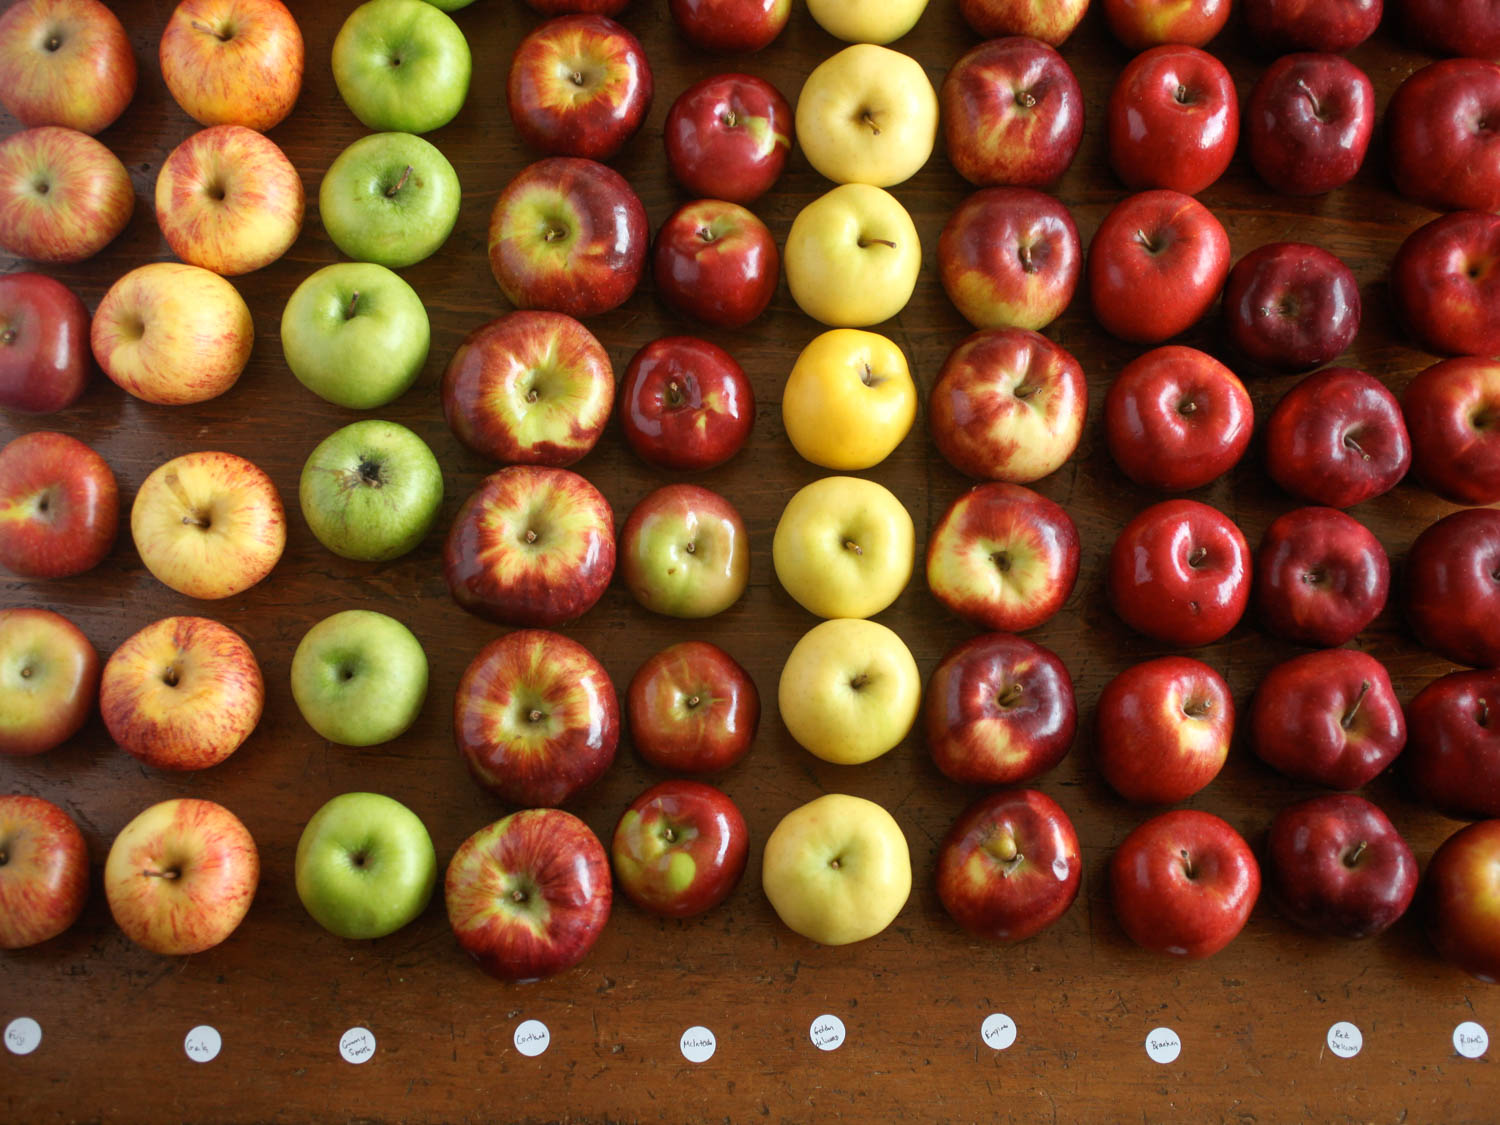
\includegraphics[width=\textwidth]{img/apples.jpg} 
		\end{figure}
	\end{minipage}
\end{frame}
\section{Sieci neuronowe}
\begin{frame}{Sieć neuronowa}
	\begin{block}{Definicja}
		\textbf{Sztuczna sieć neuronowa} --  ogólna nazwa struktur matematycznych i ich programowych lub sprzętowych modeli, realizujących obliczenia lub przetwarzanie sygnałów poprzez rzędy elementów, zwanych sztucznymi neuronami, wykonujących pewną podstawową operację na swoim wejściu.\\
		\vspace{5mm}
		\hspace*\fill{\scriptsize https://pl.wikipedia.org/wiki/Sieć\_neuronowa}
	\end{block}	
\end{frame}
\subsection{Neuron}
\begin{frame}{Klasyfikator liniowy jako najprostszy neuron}
	\begin{minipage}[t]{0.45\linewidth}
		\vfill
		\begin{figure}
			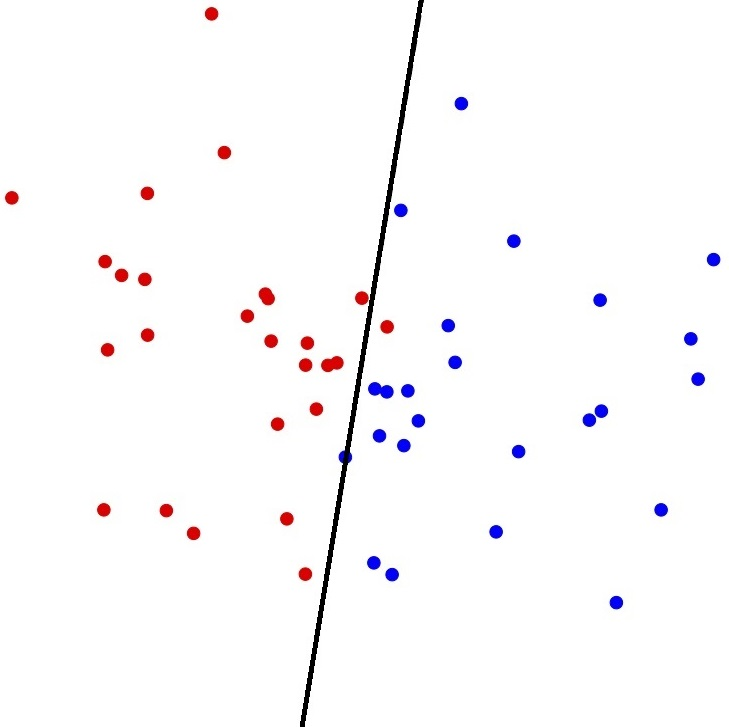
\includegraphics[height=0.6\textheight,frame]{img/linear_classifier.jpg}
			\caption{prosty klasyfikator liniowy}
		\end{figure}	
	\end{minipage}%
	\hfill
	\begin{minipage}[t]{0.45\linewidth}
		\vfill
		\begin{figure}
			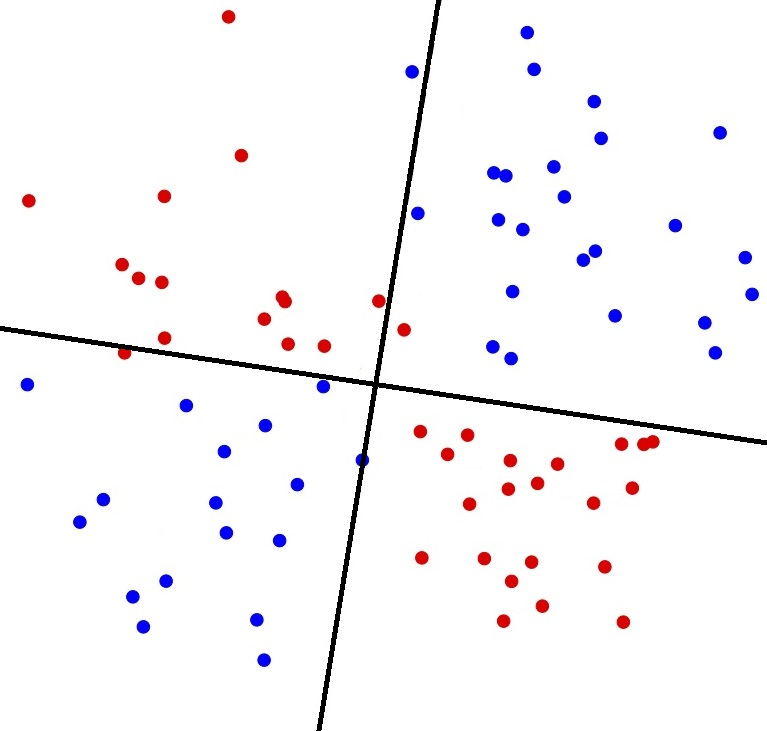
\includegraphics[height=0.6\textheight,frame]{img/xor_classifier.jpg}
			\caption{klasyfikator złożony z~3~klasyfikatorów liniowych}
		\end{figure}
	\end{minipage}
\end{frame}
\begin{frame}{Model sieci}
	\begin{minipage}[t]{0.6\linewidth}
		\vfill
		\begin{itemize}
			\item Warstwa wejściowa - neurony zaznaczone na niebiesko.
			\item Warstwa pierwsza - położenie klasyfikowanego punktu względem przedstawionych linii (patrz poprzedni slajd).
			\item Warstwa wyjściowa - określenie klasy (koloru) punktu na podstawie położenia względem obu linii.
		\end{itemize}	
	\end{minipage}%
	\hfill
	\begin{minipage}[t]{0.3\linewidth}
		\vfill
		\begin{figure}
			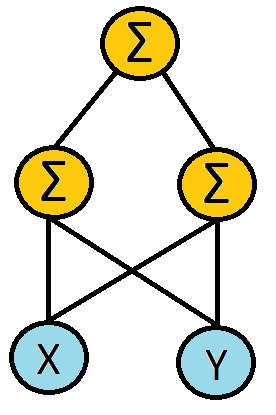
\includegraphics[height=0.6\textheight]{img/model_sieci.jpg}
		\end{figure}
	\end{minipage}
\end{frame}
\subsection{Funkcja aktywacji}
\begin{frame}{Funkcja liniowa}
	$f(x)=x$
	\begin{center}
		\begin{tikzpicture}
		\begin{axis}[
		scale only axis, % The height and width argument only apply to the actual axis
		height=5cm,
		xtick={-1,1},
		width=\textwidth,
		axis x line=center, axis y line=center,
		xlabel=$x$,
		ylabel=$f(x)$
		]
		\addplot [
			domain=-1.1:1.1,
			color=red
		]{x};
		\end{axis}
		\end{tikzpicture}
	\end{center}
\end{frame}
\begin{frame}{Funkcja progowa}
	\begin{equation*}
	f(x) =
	\begin{cases}
	0 & x<0, \\
	1 & \textrm{w p.p.}
	\end{cases}
	\end{equation*}

	\begin{center}
		\begin{tikzpicture}
		\begin{axis}[
		scale only axis, % The height and width argument only apply to the actual axis
		height=4cm,
		xmin=-3,xmax=3,
		ymin=-1.1,ymax=1.5,
		axis x line=center,
		axis y line=center,
		xtick={-3,3},
		ytick={0,1},
		xlabel=$x$,
		ylabel=$f(x)$]
		\addplot[red, samples=1000] {(x>=0)};
		\end{axis}
		\end{tikzpicture}
	\end{center}
\end{frame}
\begin{frame}{Obcięta funkcja liniowa}
	\begin{equation*}
	f(x) = \begin{cases}
	-1 & x<-1, \\
	x & -1\leq x < 1, \\
	1 & \textrm{w p.p.}
	\end{cases}
	\end{equation*}
	
	\begin{center}
		\begin{tikzpicture}
		\begin{axis}[
		scale only axis, % The height and width argument only apply to the actual axis
		height=4cm,
		xmin=-3,xmax=3,
		ymin=-1.2,ymax=1.5,
		axis x line=center,
		axis y line=center,
		xtick={-1,1},
		ytick={-1,1},
		xlabel=$x$,
		ylabel=$f(x)$]
		\addplot[red, samples=1000] {-1*(x<-1)+x*(-1<=x)*(x<1)+1*(x>=1)};
		\end{axis}
		\end{tikzpicture}
	\end{center}
\end{frame}
\begin{frame}{Funkcja sigmoidalna}
	\begin{equation*}
	f(x) = \frac{1}{1+e^{-x}}
	\end{equation*}
	
	\begin{center}
		\begin{tikzpicture}
		\begin{axis}[
		scale only axis, % The height and width argument only apply to the actual axis
		height=4cm,
		xmin=-10,xmax=10,
		ymin=-1.1,ymax=1.5,
		axis x line=center,
		axis y line=center,
		xtick={-10,10},
		ytick={0,1},
		xlabel=$x$,
		ylabel=$f(x)$]
		\addplot[red, domain=-10:10] {1/(1+e^(-x))};
		\end{axis}
		\end{tikzpicture}
	\end{center}
\end{frame}
\begin{frame}{Funkcja rampy (\textit{ang.~ramp function})}
	\begin{equation*}
	f(x) = max(0,x)
	\end{equation*}
	\begin{center}
		\begin{tikzpicture}
		\begin{axis}[
		scale only axis, % The height and width argument only apply to the actual axis
		height=4cm,
		xmin=-3,xmax=3,
		ymin=-1.1,ymax=1.5,
		axis x line=center,
		axis y line=center,
		xtick={-10,10},
		ytick={0,1},
		xlabel=$x$,
		ylabel=$f(x)$]
		\addplot[red, domain=-3:3] {max(0,x)};
		\end{axis}
		\end{tikzpicture}
	\end{center}
\end{frame}
\begin{frame}{Softplus}
	\begin{equation*}
	f(x) = ln(1 + e^x)  \hspace{1cm} f'(x) = \frac{1}{1 + e^{-x}}
	\end{equation*}
	\begin{center}
		\begin{tikzpicture}
		\begin{axis}[
		scale only axis, % The height and width argument only apply to the actual axis
		height=4cm,
		xmin=-4,xmax=4,
		ymin=-1.1,ymax=1.5,
		axis x line=center,
		axis y line=center,
		xtick={-10,10},
		ytick={0,1},
		xlabel=$x$,
		ylabel=$f(x)$]
		\addplot[red, domain=-4:4] {ln(1 + e^x)};
		\end{axis}
		\end{tikzpicture}
	\end{center}
\end{frame}


\subsection{Rodzaje sieci neuronowych}
\begin{frame}{Przykładowe rodzaje sieci neuronowych}
	\begin{itemize}
		\item prosta sieć typu Feed-Forward,
		\item sieć rekurencyjna,
		\item samoorganizująca się sieć Kohonena,
		\item Ograniczona Maszyna Boltzmanna (RBM,~\textit{ang.~Restricted~Boltzmann~Machine}),
		\item sieć splotowa.
	\end{itemize}
	Różne rodzaje sieci mogą być ze sobą łączone.
\end{frame}

\subsection{Sieć splotowa}
\begin{frame}{Filtr splotowy}
	\begin{figure}
		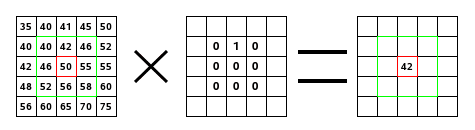
\includegraphics[height=0.6\textheight, width=\linewidth, keepaspectratio] {img/convolutional_filter.png}
		\caption{https://docs.gimp.org/en/plug-in-convmatrix.html}
	\end{figure}
\end{frame}

\begin{frame}{Filtr wyostrzający}
	\begin{minipage}[t]{0.3\linewidth}
		\vfill
		\begin{figure}
			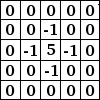
\includegraphics[width=\linewidth]{img/convolution-sharpen.png}
			\caption{https://docs.gimp.org/en/plug-in-convmatrix.html}
		\end{figure}	
	\end{minipage}%
	\hfill
	\begin{minipage}[t]{0.6\linewidth}
		\vfill
		\begin{figure}
			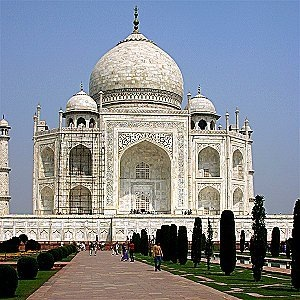
\includegraphics[width=\linewidth, height=0.7\textheight, keepaspectratio]{img/taj-sharpen.jpg}
			\caption{https://docs.gimp.org/en/plug-in-convmatrix.html}
		\end{figure}
	\end{minipage}
\end{frame}

\begin{frame}{Filtr rozmywający}
	\begin{minipage}[t]{0.3\linewidth}
		\vfill
		\begin{figure}
			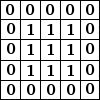
\includegraphics[width=\linewidth]{img/convolution-blur.png}
			\caption{https://docs.gimp.org/en/plug-in-convmatrix.html}
		\end{figure}	
	\end{minipage}%
	\hfill
	\begin{minipage}[t]{0.6\linewidth}
		\vfill
		\begin{figure}
			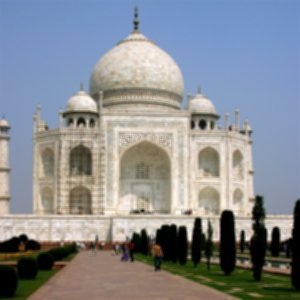
\includegraphics[width=\linewidth, height=0.7\textheight, keepaspectratio]{img/taj-blur.jpg}
			\caption{https://docs.gimp.org/en/plug-in-convmatrix.html}
		\end{figure}
	\end{minipage}
\end{frame}

\begin{frame}{Filtr wykrywający krawędzie}
	\begin{minipage}[t]{0.3\linewidth}
		\vfill
		\begin{figure}
			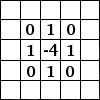
\includegraphics[width=\linewidth]{img/convolution-edge-detect.png}
			\caption{https://docs.gimp.org/en/plug-in-convmatrix.html}
		\end{figure}	
	\end{minipage}%
	\hfill
	\begin{minipage}[t]{0.6\linewidth}
		\vfill
		\begin{figure}
			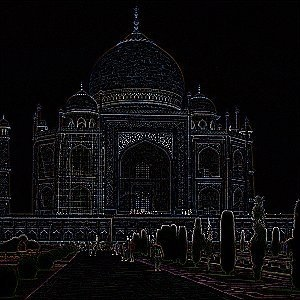
\includegraphics[width=\linewidth, height=0.7\textheight, keepaspectratio] {img/taj-edge-detect.jpg}
			\caption{https://docs.gimp.org/en/plug-in-convmatrix.html}
		\end{figure}
	\end{minipage}
\end{frame}

\begin{frame}{Jak działa sieć splotowa}
	\begin{itemize}
		\item wykorzystuje wiele filtrów splotowych o różnych maskach,
		\item wagi każdego z filtrów są wstępnie inicjowane losowo, a~następnie obliczane w procesie uczenia,
		\item wyniki zastosowania splotów to~również obrazki (tzw.~mapy~cech),
		\item mapy cech poddawane są działaniu kolejnych filtrów~spolotowych w następnych warstwach sieci.
	\end{itemize}
\end{frame}
\begin{frame}{Warstwa wejściowa}
	\begin{figure}
		
\includegraphics[width=\linewidth, height=0.7\textheight, keepaspectratio] {img/hierarchical-learning1.jpg}
		\caption{www.andrewng.org}
	\end{figure}
\end{frame}
\begin{frame}{Wykrywanie prostych elementów}
	\begin{figure}
		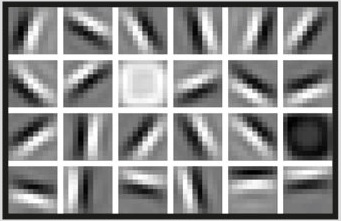
\includegraphics[width=\linewidth, height=0.7\textheight, keepaspectratio] {img/hierarchical-learning2.jpg}
		\caption{www.andrewng.org}
	\end{figure}
\end{frame}
\begin{frame}{Wykrywanie bardziej złożonych elementów }
	\begin{figure}
		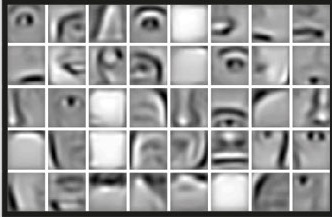
\includegraphics[width=\linewidth, height=0.7\textheight, keepaspectratio] {img/hierarchical-learning3.jpg}
		\caption{www.andrewng.org}
	\end{figure}
\end{frame}
\begin{frame}{Wykrywanie jeszcze bardziej złożonych elementów }
	\begin{figure}
		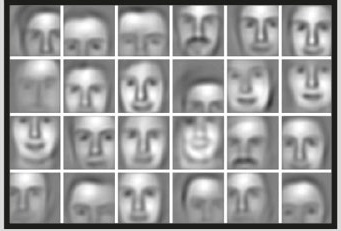
\includegraphics[width=\linewidth, height=0.7\textheight, keepaspectratio] {img/hierarchical-learning4.jpg}
		\caption{www.andrewng.org}
	\end{figure}
\end{frame}

\begin{frame}{Fazy przetwarzania obrazu przez sieć}
	\begin{enumerate}
		\item splot,
		\item normalizacja,
		\item próbkowanie,
		\item powtórzenie kroków 1-3 wiele razy,
		\item warstwa (1 lub więcej) w pełni połączona.
	\end{enumerate}
\end{frame}

\begin{frame}{Faza I - Splot}
	\begin{figure}
		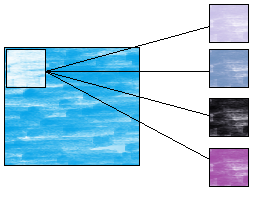
\includegraphics[width=\linewidth, height=0.7\textheight, keepaspectratio] {img/convolution.png}
	\end{figure}
\end{frame}

\begin{frame}{Faza II - Próbkowanie (\textit{ang.~subsampling})}
	\begin{minipage}[t]{0.6\linewidth}
		\begin{itemize}
			\item szybko rosnący rozmiar danych wyjściowych dla kolejnych warstw,
			\item zmniejszanie rozmiaru danych przez zmniejszanie obrazków,
			\item average pooling i max-pooling.
		\end{itemize}
	\end{minipage}%
	\hfill
	\begin{minipage}[t]{0.3\linewidth}
		\vfill
		\begin{figure}
			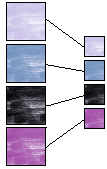
\includegraphics[width=\linewidth, height=0.7\textheight, keepaspectratio] {img/pooling.png}
		\end{figure}
	\end{minipage}
\end{frame}

\begin{frame}{Faza końcowa}
	\begin{figure}
		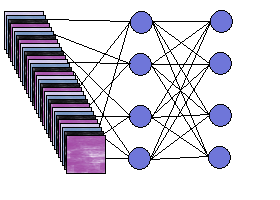
\includegraphics[width=\linewidth, height=0.7\textheight, keepaspectratio] {img/fully_connected_layer.png}
	\end{figure}
\end{frame}

\begin{frame}{Problemy w sieciach splotowych}
	\begin{itemize}
		\item Zanikający gradient przy wielu warstwach
		\begin{itemize}
			\item uczenie wstępne,
			\item zastosowanie funkcji rampy lub softplus.
		\end{itemize}
		\item koadaptacja neuronów $\rightarrow$ drop-out,
		\item underfitting i overfitting
		\begin{itemize}
			\item zmiana struktury sieci (liczba warstw, liczba neuronów, rozkład neuronów w warstwach)
			\item uczenie wstępne.
		\end{itemize}
	\end{itemize}
\end{frame}

\section{Tensorflow}
\begin{frame}{Czym jest Tensorflow}
	\begin{itemize}
		\item biblioteka do Pythona,
		\item wykorzystuje grafy przepływu danych do efektywnego wykonywania obliczeń
		\begin{itemize}
			\item węzły - operacje matematyczne,
			\item krawędzie - tensory wymieniane pomiędzy operacjami matematycznymi.
		\end{itemize}
		\item możliwość uruchamiania kodu na wielu procesorach (CPU), wielu kartach graficznych (GPU),
		\item możliwość uruchamiania kodu zarówno na wielu urządzeniach (serwery, urządzenia mobilne,
		komputery stacjonarne) przy wykorzystaniu tego samego API,
		\item stworzony w ramach projektu Google's Machine Intelligence (projekt z Google Brain).
	\end{itemize}
\end{frame}
\begin{frame}{Graf przepływu danych}
	\begin{figure}
		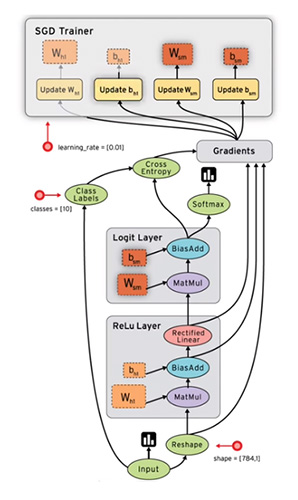
\includegraphics[height=0.85\textheight, keepaspectratio] {img/data-flow-graph.jpg}
	\end{figure}
\end{frame}

\section{Podsumowanie}
\begin{frame}{Podsumowanie}
  \begin{itemize}
    \item gwałtowny rozwój technologii i jego implikacje,
    \item uczenie nadzorowane vs. nienadzorowane,
    \item sieci neuronowe,
    \item przykładowe funkcje aktywacji,
    \item przykładowe typy sieci,
    \item filtry splotowe,
    \item zasada działania sieci splotowych,
    \item tensorflow.
  \end{itemize}
\end{frame}
\begin{frame}{Ciekawe odnośniki}
	\begin{itemize}
		\item tworzenie i wizualizacja działania sieci neuronowej:\\
		http://playground.tensorflow.org/
		\item gra w kalambury ze Sztuczną Inteligencją:\\
		https://quickdraw.withgoogle.com
		\item generowanie opisów do obrazków:\\
		http://deeplearning.cs.toronto.edu/i2t
		\item generowanie tekstu pisanego ręcznie:\\
		http://www.cs.toronto.edu/~graves/handwriting.html
		
	\end{itemize}
\end{frame}
\begin{frame}{Bibliografia}
	\begin{itemize}
		\item Cichosz P., Systemy uczące się, WNT Warszawa, 2000,
		\item https://www.tensorflow.org/
		\item http://karpathy.github.io/,
		\item https://en.wikipedia.org/wiki/AlphaGo,
		\item https://pl.wikipedia.org/wiki/Uczenie\_nadzorowane,
		\item https://pl.wikipedia.org/wiki/Uczenie\_nienadzorowane,
		\item https://pl.wikipedia.org/wiki/Sieć\_neuronowa,
		\item https://docs.gimp.org/en/plug-in-convmatrix.html,
		\item http://www.andrewng.org/.
	\end{itemize}
\end{frame}

\begin{frame}{Pytania}
  \begin{figure}
    
\includegraphics[width=0.35\textwidth]{img/question-mark-red.png} 
  \end{figure}
\end{frame}

\end{document}
